\subsection{Module Interconnection}

By interconnecting the modules derived in the last chapter, datapaths are created. By forming cycles in the datapaths, the outputs of previous operations can be used as an input to new ones. The datapaths can also be multiplexed, i.e an output can dynamically be configured to be drive by one of multiple inputs. By doing so, the machine can execute different operations using identical hardware, depending on the configuration of the datapath. 

\begin{figure}[H]
    \centering
    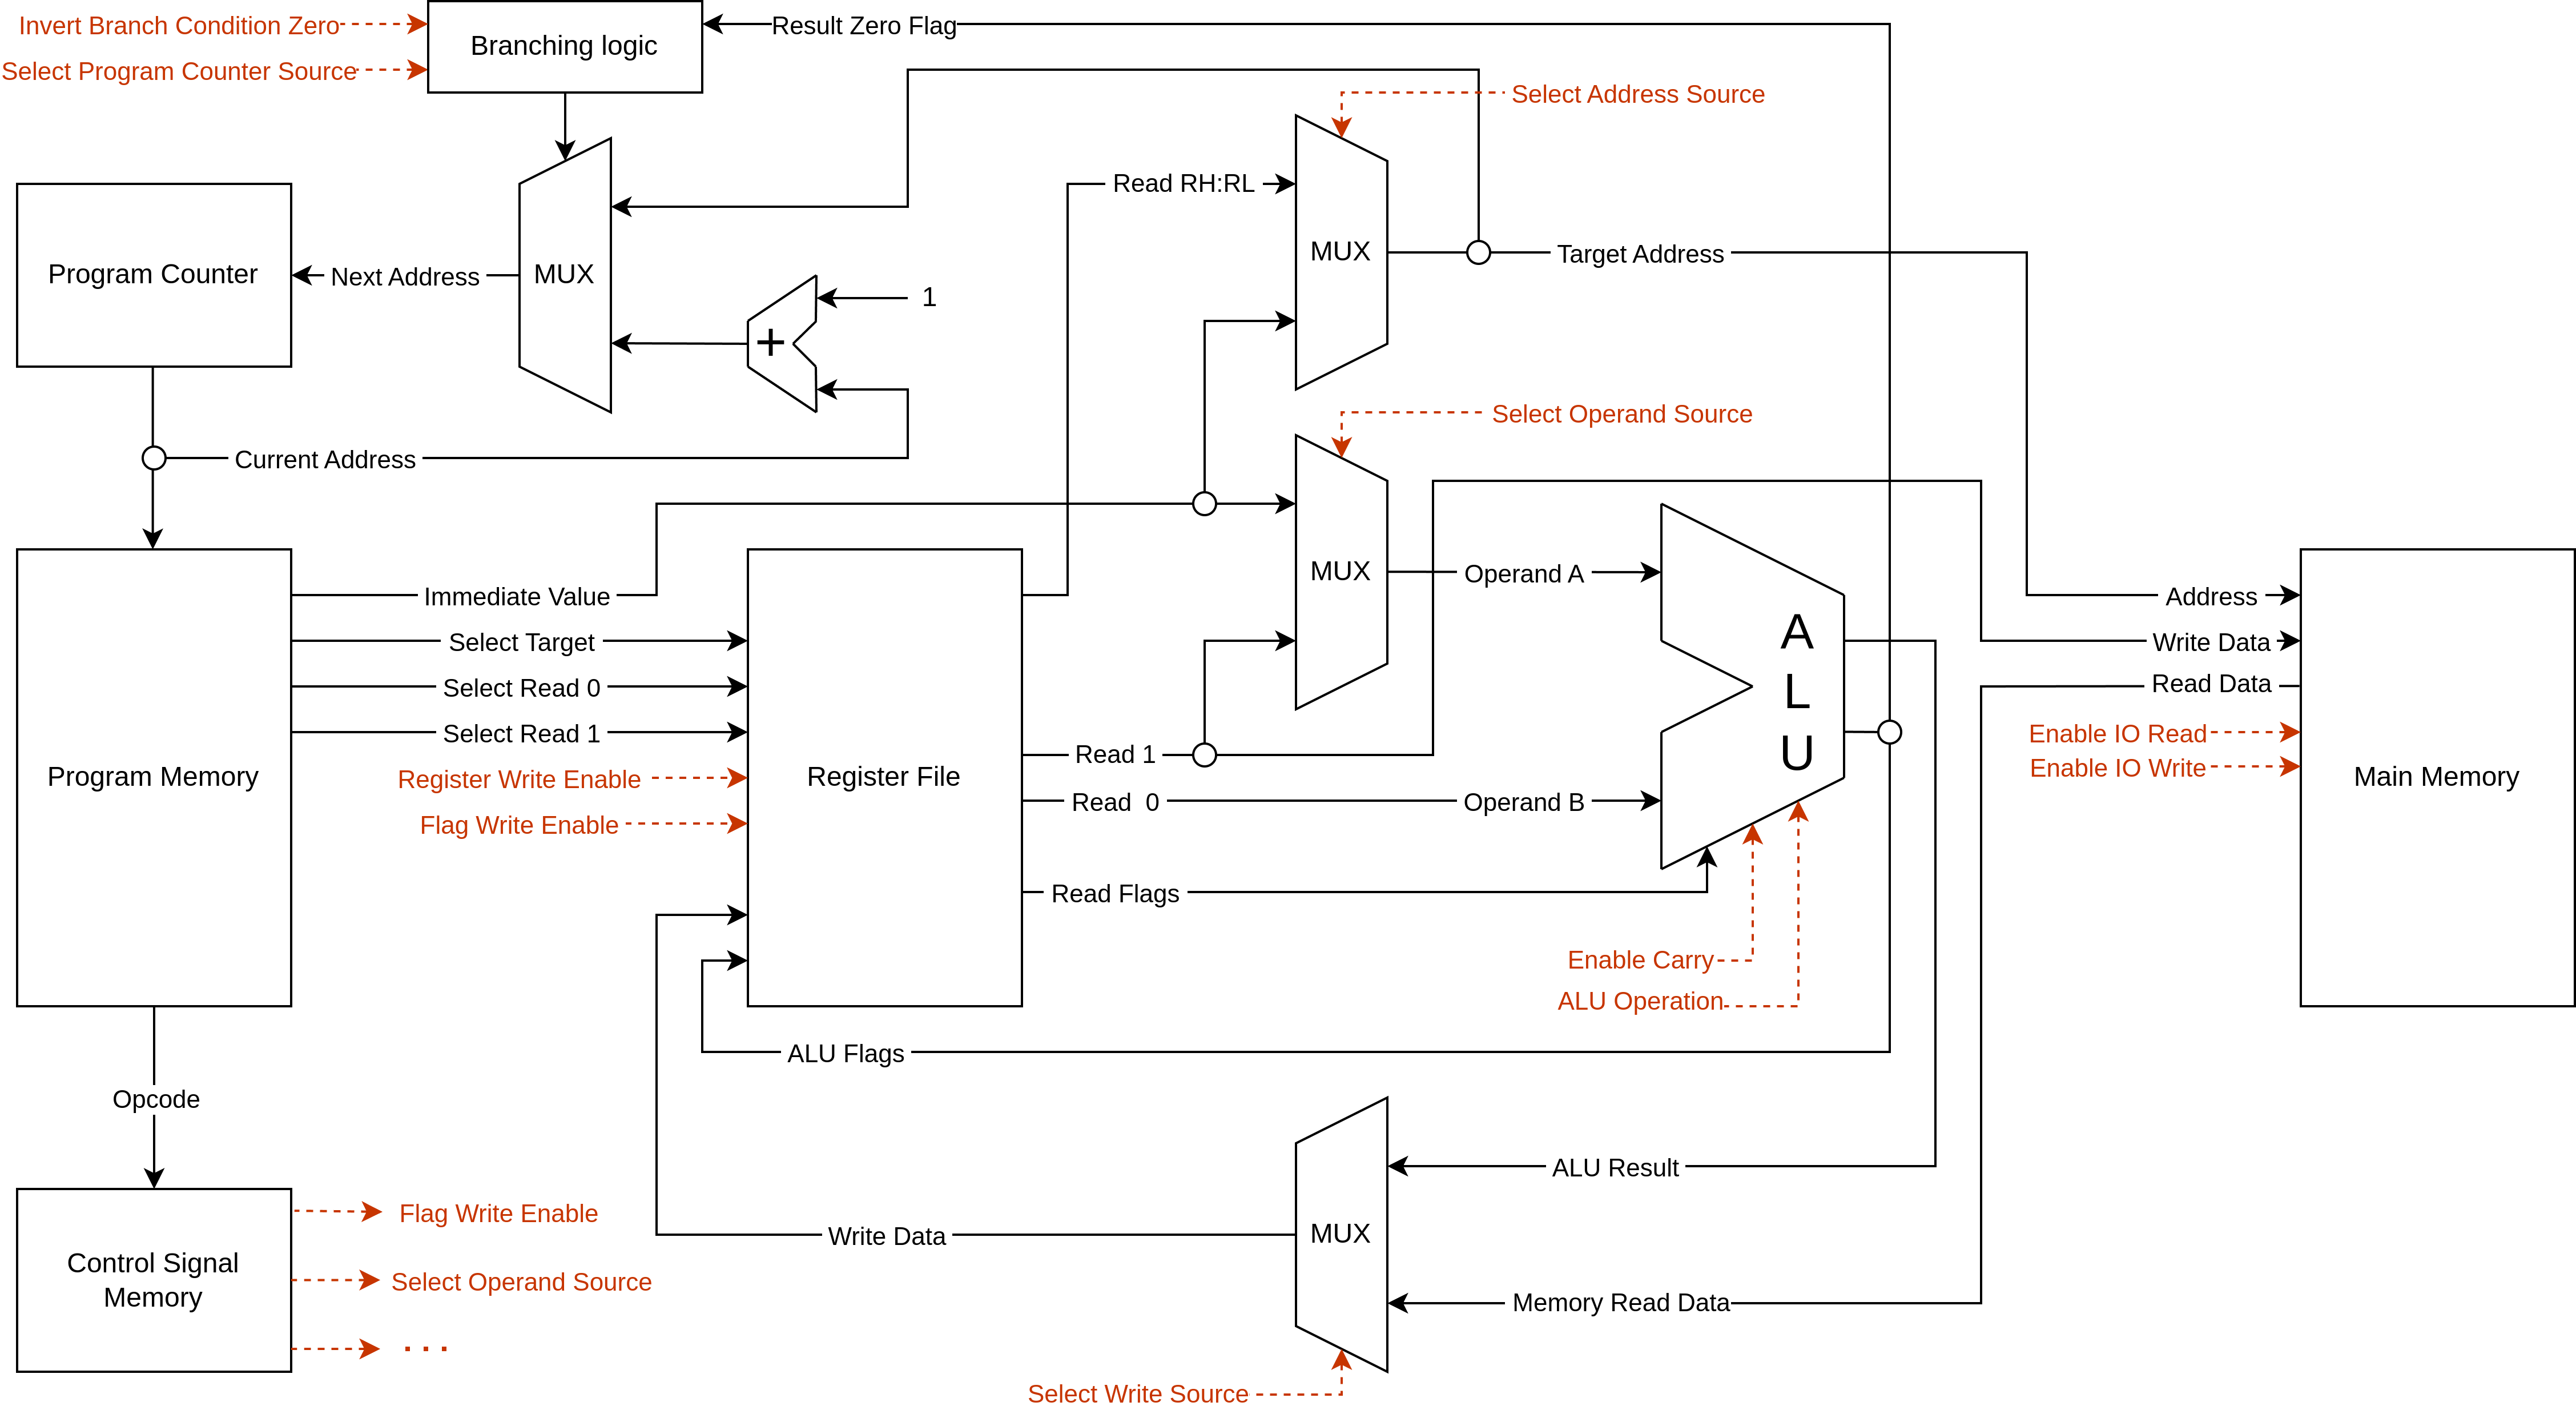
\includegraphics[width=1.0\textwidth]{images/drawio/datapath.png}  % Replace with your image file
    \caption{Datapath of a possible implementation of the AVA architecture, omitting clock signals and external interfaces. Data lines are drawn in solid black, dotted red lines indicate control signals}
    \label{fig:implementation_interconnection_datapath}
\end{figure}

\autoref{fig:implementation_interconnection_datapath} shows the datapath of a possible implementation. It makes the assumption that all modules work as described in the last chapter. The clock generation logic and clock signals are omitted for clarity of the datapath. There are 11 control signals in total. Since the \ac{alu} operation is encoded using three bits and the ``halt'' signal is omitted, there is a total of 15 individual control signal lines. 